\documentclass[../main.tex]{subfiles}
\begin{document}
\subsection*{Quantum Numbers}
The energy eigenstates of the hydrogen atom are states of definite energy, magnitude of angular momentum, and z component of angular momentum. The values of those quantities are labeled by the quantum numbers $n$, $l$, and $m_l$, respectively. These three quantum numbers must be integers, and the spin quantum number $m_s$ must be $-1/2$ (spin-up) or $-1/2$ (spin-down). Other restrictions are given below.
\begin{center}
    \begin{tabular}{| p{0.09\textwidth} | p{0.25\textwidth} | p{0.2\textwidth} | p{0.3\textwidth}|}
        \hline
        Letter&Name&Range&Physical interpretation\\
        \hline
        $n$&Principal quantum number&$1 \leq n <\infty$&$E_n = -(1/n^2) Ry$, with $ (1 \;Ry \approx 13.6$ eV)\\
        $l$&Angular momentum quantum number&$0 \leq l \leq n - 1$ &$ |\overrightarrow{L}| = \sqrt{l(l + 1) }\hbar$\\
        $m_l$&Magnetic quantum number&$-l \leq m_l \leq l$&$L_z = m_l\hbar$\\
        $m_s$&Spin quantum number&$m_s = \pm 1/2$&$S_z = m_s\hbar$\\\hline
    \end{tabular}
\end{center}

\textbf{Principal Quantum Number \emph{n}.} The term “principal quantum number” refers to the fact that $n$ determines energy: each eigenstate $\psi_{nlm_l}$  has energy $E_n = -(1/n2)$ Ry, where 1 Ry $\approx$ 13.6 eV is a unit of energy called a “rydberg.” So the ground state of hydrogen has energy -1 Ry $\approx$ -13.6 eV, the first excited state has energy -(1/4) Ry $\approx$ -3.4 eV, and so on.

\textbf{Angular Momentum Quantum Number \emph{l}.} $l$ controls the magnitude of the total angular momentum of the electron about the nucleus is $L = \sqrt{l(l + 1)} \hbar$.

\textbf{Magnetic Quantum Number $\boldsymbol{m_l}$.}  While $l$ determines the magnitude of the angular momentum vector, $m_l$ determine the z component of the angular momentum $L_z = m_l \hbar$. The name comes from the fact that the simplest way to measure a particular component of the angular momentum of a charged particle is to measure the magnetic field it creates.

\textbf{Spin $\boldsymbol{m_s}$.} In 1924 Pauli suggested that each electron in an atom has a fourth quantum number that can only take on two possible values. He gave no physical explanation for this new electron property, which he called a “two-valuedness not describable classically.” Consider a ball spinning about its own axis, except it is not a ball and it is not spinning.

For every electron, the magnitude of spin is $\sqrt{s(s + 1)}\hbar=\sqrt{3/4}\hbar$, with values of $-1/2$ or $+1/2$. The z component of the spin is therefore $L_z= m_s\hbar=\pm(1/2)\hbar$.

Any particle with half-integer spin is a fermion, for example electrons, protons, and neutrons. Any particle with integer spin is a boson, for example photons. Every particle can be classified as either a “fermion,” meaning it obeys the Pauli exclusion principle, or a “boson,” meaning it does not. 

The energy eigenvalues of a hydrogen atom depend only on n (to a very good approximation). The  following formulas use $m_e$ and $e$ for the electron mass and charge, respectively
\begin{multline*}
    E_n=-\frac{m_ee^4}{32\pi^2\epsilon_0^2
    \hbar^2n^2}=-\frac{1}{2n^2}m_ec^2\alpha^2 = -\frac{1}{n^2}\text{Ry}\\
    = -\frac{1}{n^2}13.6 \text{eV}=\frac{1}{n^2}2.18\times 10^{-18}\text{J}
\end{multline*}
where $\alpha$ is fine structure constant
\begin{equation*}
    \alpha \equiv \frac{1}{4\pi\epsilon_0}\frac{e^2}{\hbar c}\approx \frac{1}{137}
\end{equation*}
For a hydrogen-like atom with $Z$ protons and one electron, the energies are
\begin{equation*}
    E_n-\frac{Z^2}{n^2}\text{Ry}
\end{equation*}

\subsection*{Energies of Different Quantum State}
\textbf{Pauli exclusion principle.} Pauli exclusion principle forbid two or more of the same type of fermion in the same quantum state as each other. That means that, in the ground state of a multielectron atom, the $Z$ electrons (fermion) fill up the $Z$ lowest-energy states.

\textbf{$\boldsymbol{n + l}$ rule.} Given two states $\psi_{nl}$, the subshell with the lower sum n + l will fill up first. In the case of a tie, the lower-n state fills first.
\begin{figure*}
    \centering
    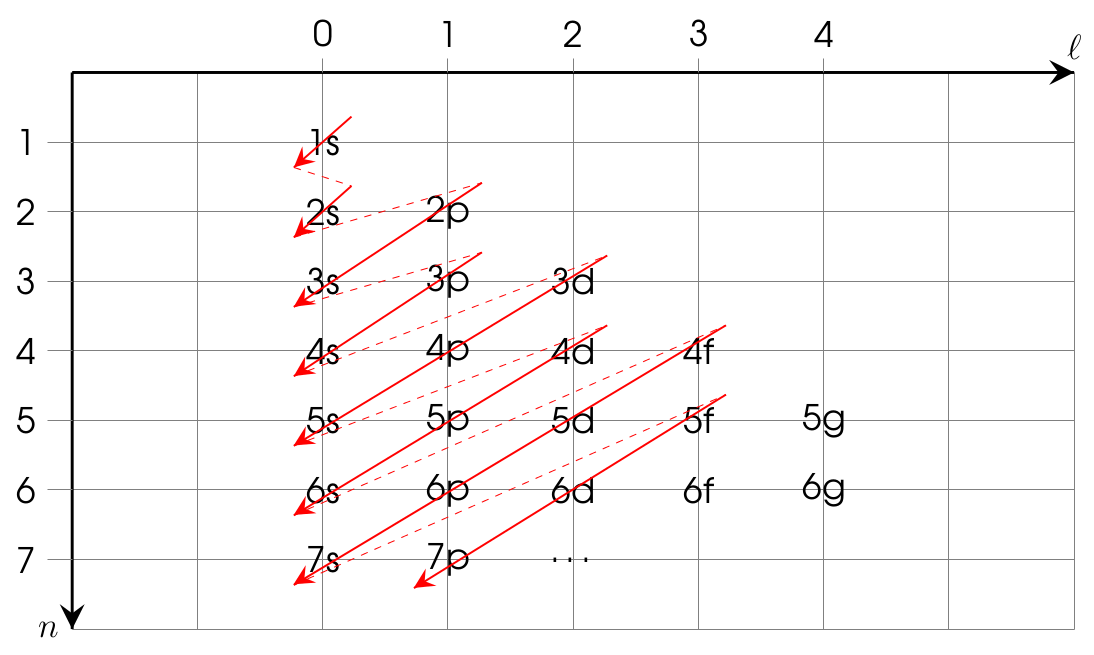
\includegraphics[width=0.5\textwidth]{../Rss/HA/Aufbau.png}
    \caption*{Figure: Perhabs the more familiar name for $n+l$ rule is Aufbau rule}
\end{figure*}

\textbf{Hund's Rule.} Because each electron can have spin up or spin down, two electrons can be in each
combination of $n$, $l$, and $m_l$. That in turn means each subshell consists of $2(2l + 1)$ degenerate states, with $2n^2$ degenerate state for each shell. Within a particular subshell, the electrons tend to end up in the states that minimize the energy level. Two nearby electrons whose spins are identical will be, on average, farther apart from each other than if they have opposite spins. The result is that electrons with identical spins shield each other from the nucleus less than electrons with different spins, so same-spin is a lower energy state than opposite-spin.

\subsection*{Energy Eigenstates}
The energy eigenstates of the hydrogen atom are of the form
\begin{equation*}
    \psi_{nlm_l} (r,\theta,\phi) = R_{nl}(r)Y^{m_l}_l (\theta,\phi).
\end{equation*}
A full specification of the quantum state of a hydrogen atom also includes the spin state (up or down) of the electron.

\subsection*{Radial Wavefunction}
The radial wavefunction is given by the following:
\begin{equation*}
    R_{nl}(r)=\sqrt{ \bigg(\frac{2}{na_0}\bigg)^3 \frac{(n - l - 1)!}{2n[(n + l)! ]^3}} \bigg(\frac{2r}{na_0}\bigg)^l \exp \biggl( - \frac{r}{na_0} \biggr) L_{n-l-1}^{2l+1}\biggl(\frac{2r}{na_0}\biggr)
\end{equation*}
where $L$ is called an associated Laguerre polynomial and is defined as
\begin{equation*}
    L_n^{k}(x) =(-1)^k\biggl(\frac{d}{dx}\biggr)^k\biggl[ e^x \frac{d^{p+k}}{dx^{p+k}}\bigl(e^{-x}x^{p+k}\bigr) \biggr]
\end{equation*}
As you know,  $k = 0$ then the above formula calls for the “zeroth derivative,” or the function itself. $ R_{nl}(r)$ is a polynomial in $r$ times a decaying exponential $e^{-r/(a_0n)}$, where $a_0$ is a constant called the “Bohr radius”
\begin{equation*}
    a_0\equiv \frac{4\pi \epsilon_0\hbar^2}{m_e e^2}\approx 5 \times 10^{-11} \;\text{m}
\end{equation*}
Here's first few Radial Wavefunctions: for $n=1$
\begin{equation*}
    R_{1,0}=2a_0^{-3/2}\exp \biggl(-\frac{r}{a_0}\biggr)
\end{equation*}
for $n=2$
\begin{align*}
    R_{2,0}&=\frac{1}{\sqrt{2}}a_0^{-3/2}\biggl(1-\frac{r}{2a_0}\biggr) \exp \biggl(-\frac{r}{2a_0}\biggr)\\
    R_{2,1}&=\frac{1}{\sqrt{24}}a_0^{-3/2} \frac{r}{a_0} \exp \biggl(-\frac{r}{2a_0}\biggr)
\end{align*}
for $n=3$
\begin{align*}
    R_{3,0}&=\frac{2}{\sqrt{27}} a_0^{-3/2} \biggl[1-\frac{2r}{3a_0}+\frac{2}{27}\biggl(\frac{r}{a_0}\biggr)^2 \biggr] \exp \biggl(-\frac{r}{3a_0}\biggr)\\
    R_{3,1}&=\frac{8}{27\sqrt{6}} a_0^{-3/2} \biggl(1-\frac{r}{6a_0}\biggr)\frac{r}{a_0} \exp \biggl(-\frac{r}{3a_0}\biggr)\\
    R_{3,2}&=\frac{4}{81\sqrt{30}} a_0^{-3/2} \biggl(\frac{r}{a_0}\biggr)^2 \exp \biggl(-\frac{r}{3a_0}\biggr)\\
\end{align*}

\subsection*{Spherical Harmonics}
Spherical harmonics are products of complex exponentials in $\phi$ and polynomials in $\cos \theta$:
\begin{equation*}
    Y_l^{m_l}(\theta, \psi)=\pm \sqrt{ \frac{2l + 1}{4\pi} \frac{(l - |m_l|)!}{(l + |m_l|)!}}P_l^{m_l}(\cos\theta) \exp (im_l\phi )
\end{equation*}
where $l$ and $m_l$ are integers and $-l \leq m_l \leq l$. The plus minus comes from $+1$ for all negative $m_l$ and all even values of $m_l$, and $-1$ for odd positive values. So the only differences between $Y^{m_l}_l$ and and $Y^{-ml}_l$ are that they have different signs if $m_l$ is odd, and the exponent in $e^{im_l\phi}$ changes sign between them. Also, P is an “associated Legendre polynomial”
\begin{equation*}
    P_l^{m_l} (x)\equiv (1-x^2)^{|m_l|/2}\biggl(\frac{d}{dx}\biggr)^{|m_l|}\biggl[ \frac{1}{2^ll!}\biggl(\frac{d}{dx}\biggr)^l(x^2-1)^l\biggr]
\end{equation*}
Not to be confused by Legendre polynomials (defined by Rodrigues formula)
\begin{equation*}
    P_l (x)\equiv \frac{1}{2^ll!}\biggl(\frac{d}{dx}\biggr)^l(x^2-1)^l
\end{equation*}
$Y^{m_l}_l$ is a polynomial in $\sin \theta$ and $\cos \theta$ multiplied by $e^{im_l\phi}$. Here's first few Spherical Harmonics: for $l=0$
\begin{equation*}
    Y_0^0=\sqrt{\frac{1}{4\pi}}
\end{equation*}
for $l=1$
\begin{align*}
    Y_1^0&=\sqrt{\frac{3}{4\pi}}\cos\theta \\
    Y_0^{\pm1}&=\mp\sqrt{\frac{3}{8 \pi}}\sin\theta e^{\pm i\phi}
\end{align*}
for $l = 2$
\begin{align*}
    Y_2^0&=\sqrt{\frac{5}{16 \pi}}(3\cos^2\theta-1) \\
    Y_2^0&=\mp\sqrt{\frac{15}{8 \pi}}\sin\theta \cos \theta e^{\pm 2i\phi}\\
    Y_2^0&=\sqrt{\frac{15}{31 \pi}}\sin^2\theta e^{\pm 2i\phi}
\end{align*}

\subsection*{Probability Distributions}
For any particle with wavefunction $\Psi$ in 3D, the probability per unit volume of finding the particle in a given region is $|\Psi|2$ . For an electron in a hydrogen atom energy eigenstate $\psi_{nlm_l}$ , probability of finding the electron between radii $r_1$ and $r_2$
\begin{equation*}
    P(r_1 \leq r \leq r_2)= \int_{r_1}^{r_2}r^2R^2\;dr
\end{equation*}
while the probability of finding the electron in a specified range of angles is
\begin{equation*}
    \int_{\theta_1}^{\theta_2}\int_{\phi_1}^{\phi_2} \sin\theta \big| Y_l^{m_l}\big|^2\;d\psi d\theta
\end{equation*}
These integrals are normalized so that
\begin{equation*}
    \int_{0}^{\infty}r^2R^2\;dr = \int_{0}^{\pi}\int_{0}^{2\pi} \sin\theta \big| Y_l^{m_l}\big|^2\;d\psi d\theta =1
\end{equation*}

\subsection*{Zeeman Effect} 
The Zeeman effect refers to the changes in atomic spectra caused by an external magnetic field. In classical electrodynamics, magnets tend to align with magnetic fields, or magnet pointing along an external magnetic field has less energy than one pointing opposite to the external field. Because an electron is negatively charged, its magnetic moment points opposite to its angular momentum. So a positive $m_l$ means its magnetic moment is pointing opposite external field, if we define positive z axis as the direction of external field. A negative $m_l$ means the electron's magnetic field is pointing with the external field, which is the preferred (low-energy) orientation.

Therefore, in an external magnetic field pointing in the positive z direction, higher $m_l$ leads to higher energy. For weak magnetic fields (neglecting spin), the Zeeman contribution to the energy of a state is
\begin{equation*}
    \Delta E=m_l\mu_BB
\end{equation*}
where $\mu_B$ is Bohr magneton
\begin{equation*}
    \mu_B=\frac{e\hbar}{2m_e}
\end{equation*}
If an atom transitions between states in which all its electron spins cancel, then you can ignore spin. In that case the splitting caused by a magnetic field is called the “normal Zeeman effect.” in the presence of an external magnetic field, the normal Zeeman effect splits the $n = 2$ to $n = 1$ transition into three separate transitions based on $\Delta m_l$. The selection rule limits which electron transitions generally occur
\begin{align*}
    \Delta l&=\pm 1\\
    \Delta m_l&=-1,0,1
\end{align*}
\end{document}

